\documentclass[11pt]{article}
\usepackage{graphicx}

\begin{document}

\title{SPS Coursework 2 Report}
\author{Michael Mafeni and Ainesh Sevellaraja}
\date{}
\maketitle

\section{Feature Selection}
We first plotted a 13x13 scatter plot for all pairwise combinations of features of the training data set, as seen below.

%in Figure \ref{fig:13x13}.
  
%\begin{figure}
%\centering
\begin{center}
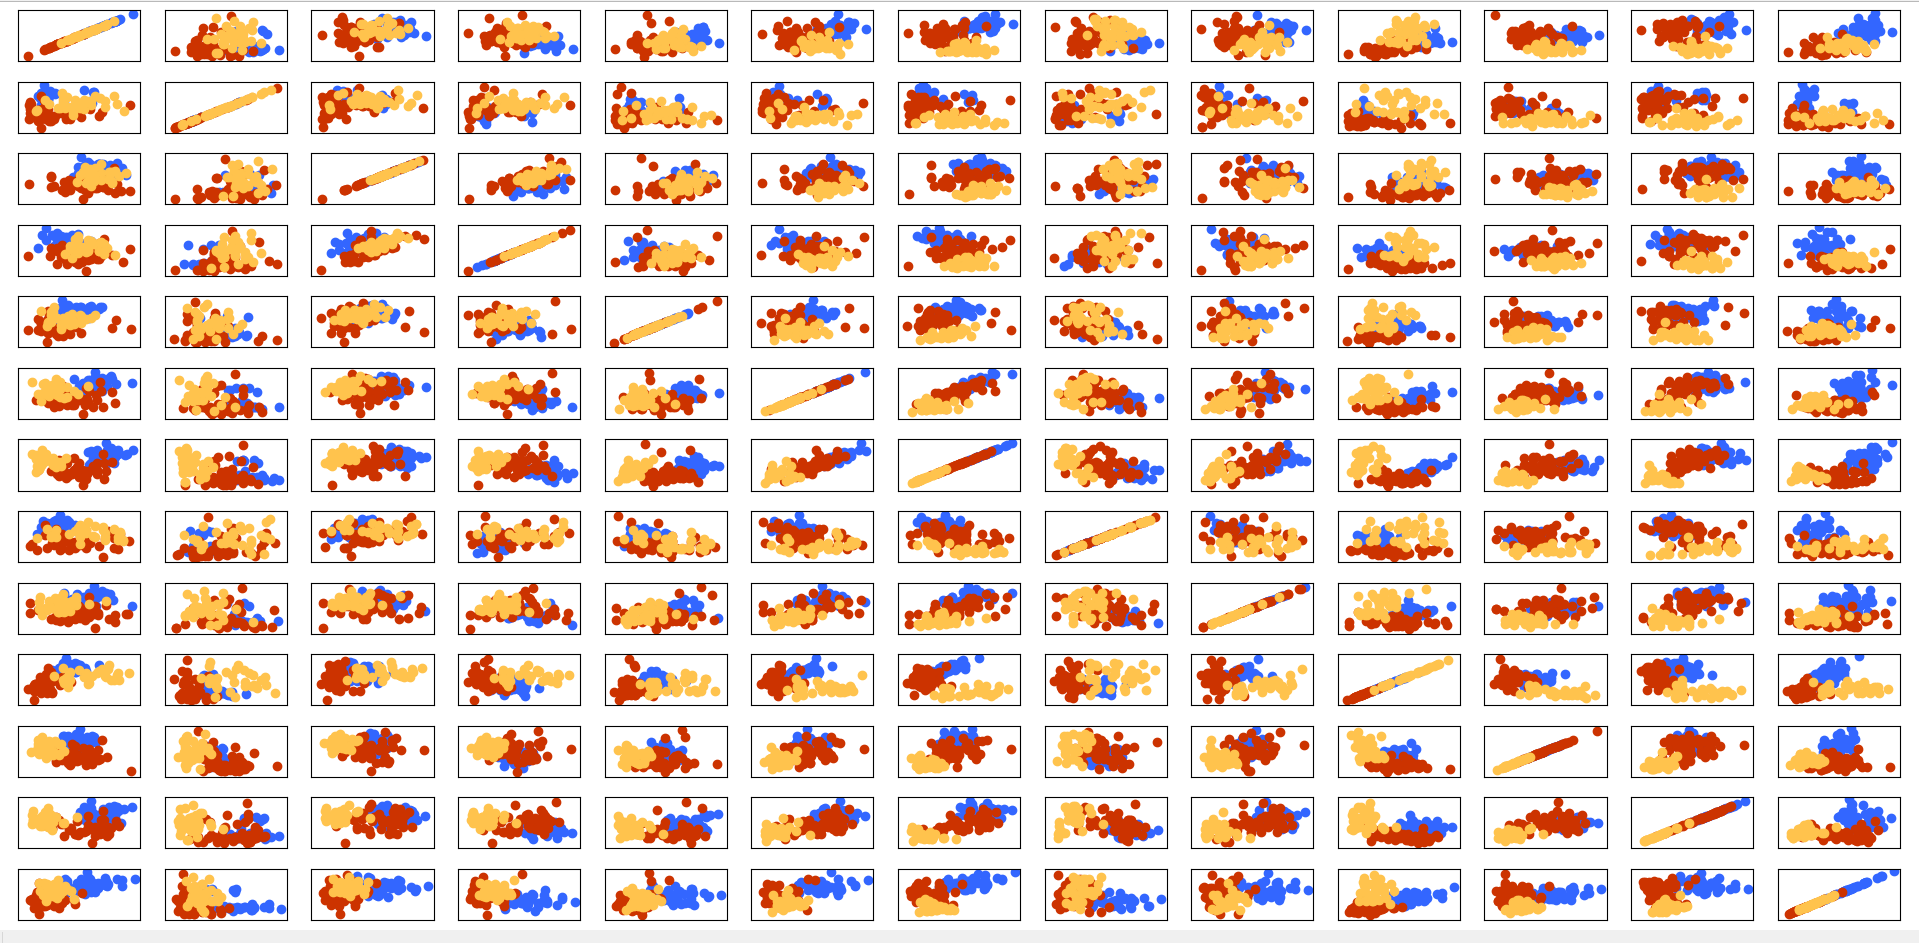
\includegraphics[scale=0.25]{feature_selection}
\end{center}
%\caption{13x13 plot of pairwise combinations of features}
%\label{fig:13x13}
%\end{figure}

Based on the plot above, we decided to select features 10 and 12 as the data separate into their classes fairly well. This can be seen in the scatter plot of feature 12 against feature 10 below. We then reduced the train set and test set to only contain features 10 and 12.
% in Figure \ref{fig:10and12}.

%\begin{figure}
%\centering
\begin{center}
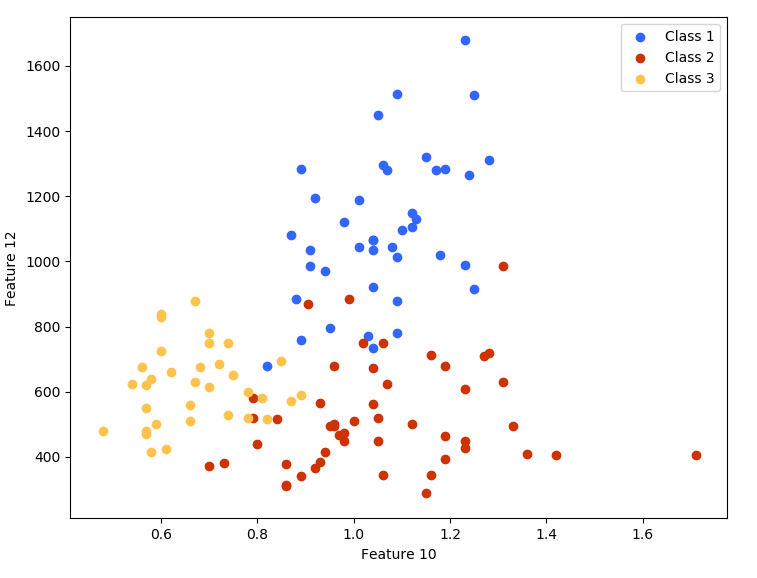
\includegraphics[scale=0.3]{features_10_12}
\end{center}
%\caption{Features 10 and 12 isolated}
%\label{fig:10and12}
%\end{figure}

\section{K-Nearest Neighbours}
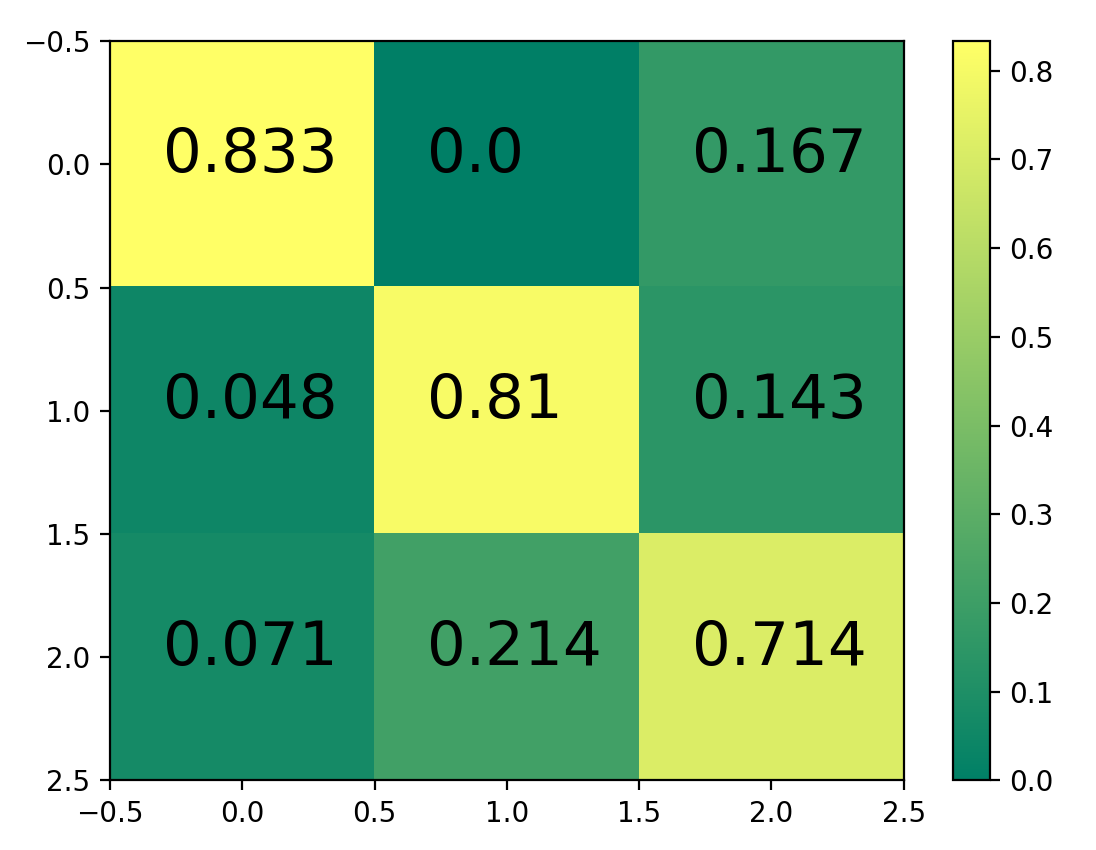
\includegraphics[scale=0.3]{Confusion_matrix(k=1)}
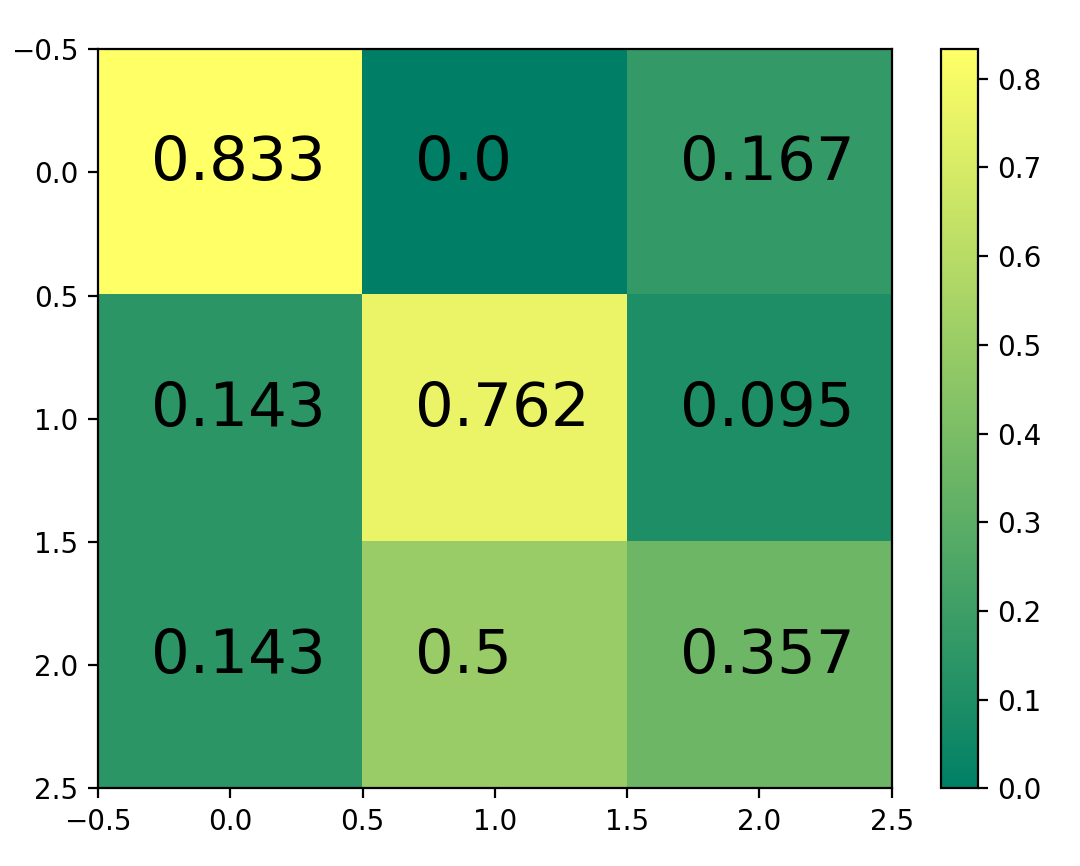
\includegraphics[scale=0.3]{Confusion_matrix(k=2)}
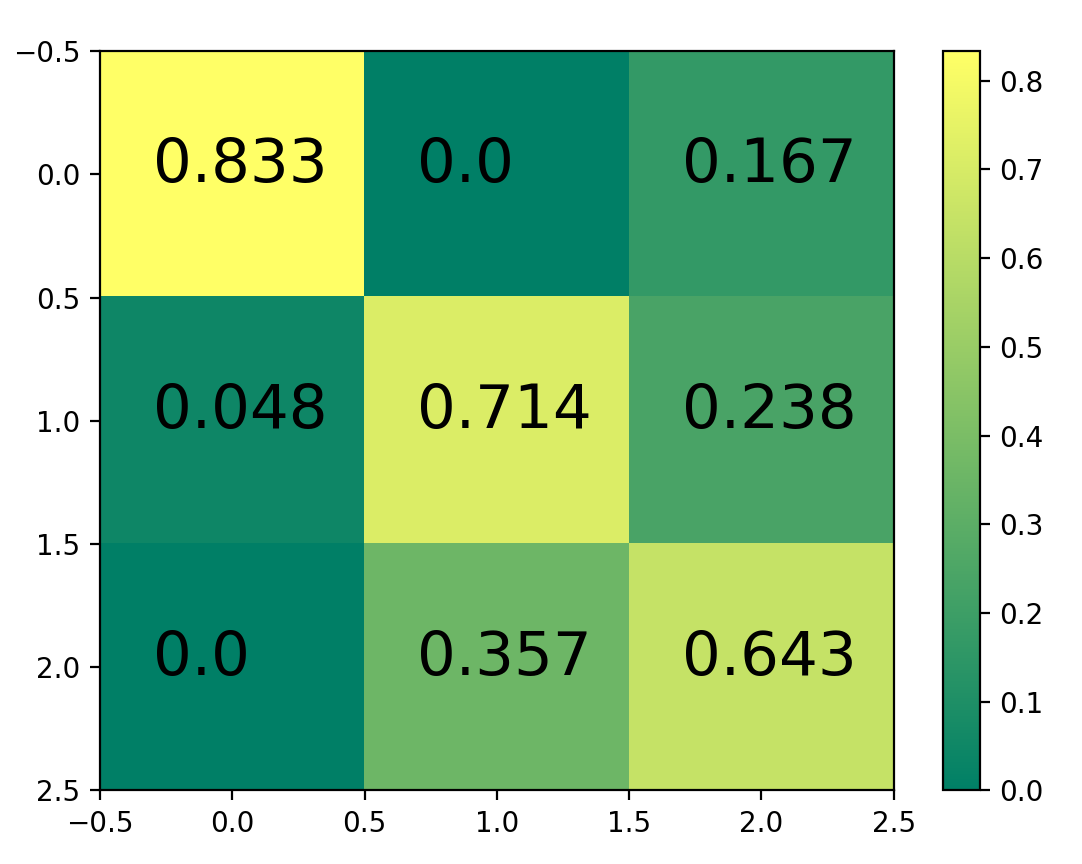
\includegraphics[scale=0.3]{Confusion_matrix(k=3)}
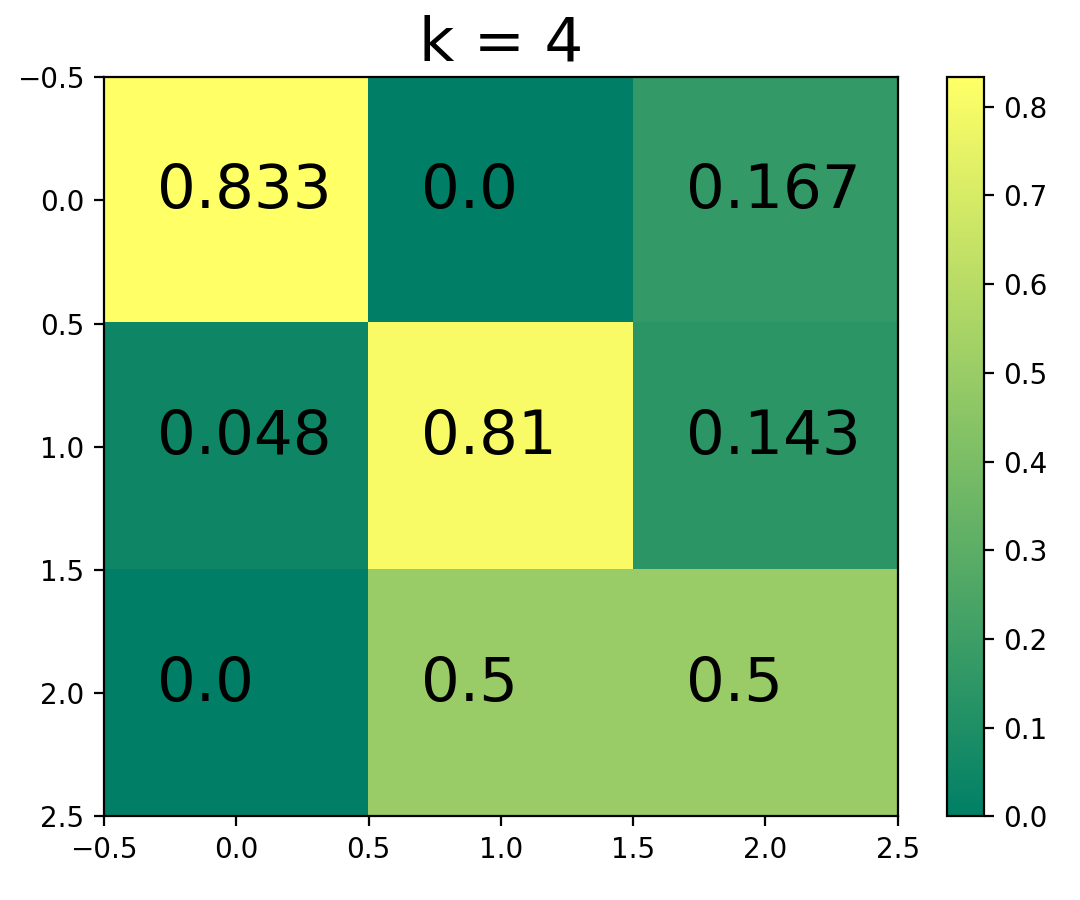
\includegraphics[scale=0.3]{Confusion_matrix(k=4)}
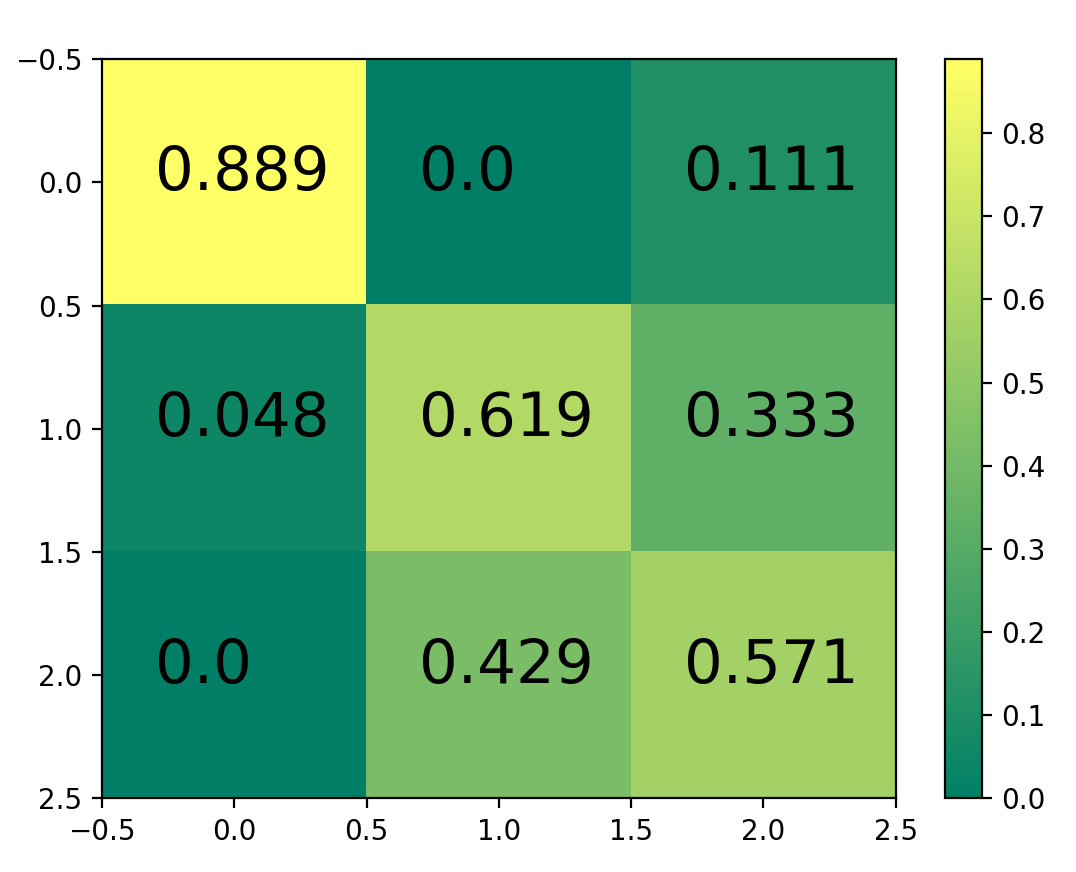
\includegraphics[scale=0.3]{Confusion_matrix(k=5)}
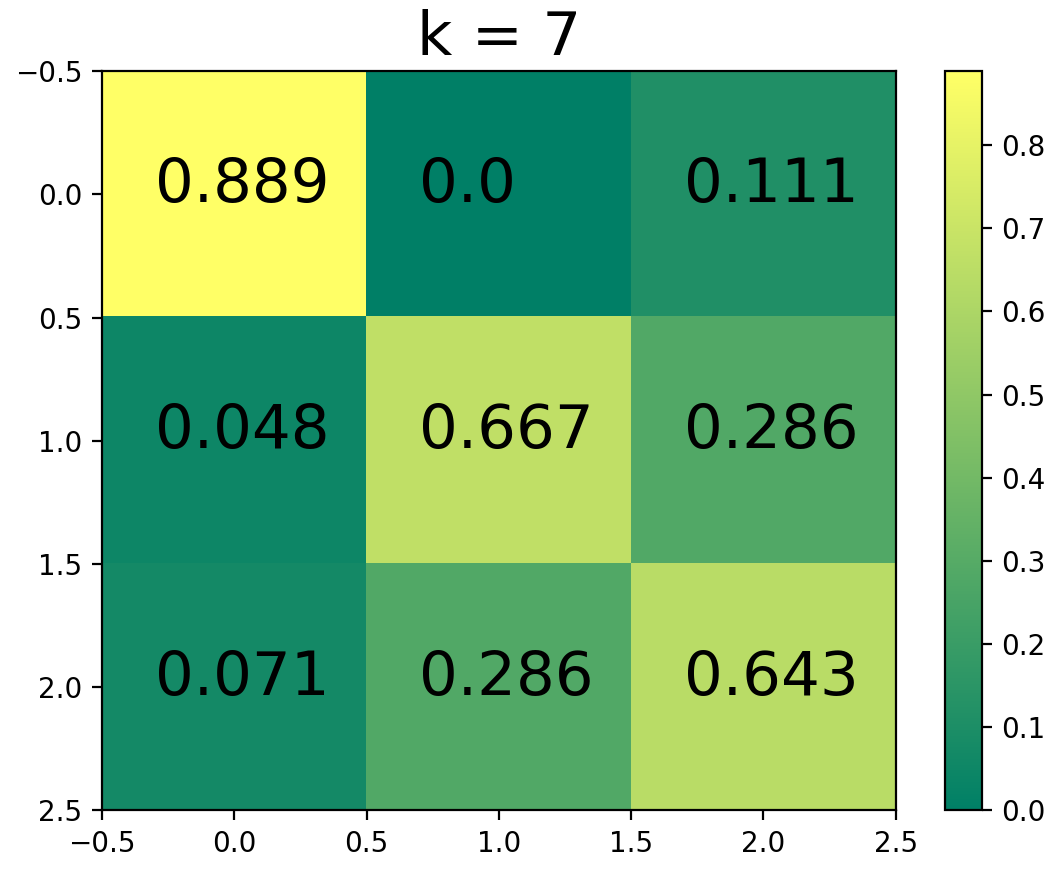
\includegraphics[scale=0.3]{Confusion_matrix(k=7)}

\section{Alternative Classifier}

\section{Use Three Features}

\section{Principal Component Analysis (PCA)}

\end{document}

